\documentclass[crop,tikz,convert={outext=.svg,command=\unexpanded{pdf2svg \infile\space\outfile}},multi=false]{standalone}

%math and margin packages
\usepackage{amsmath,amsfonts,amssymb,amsthm}
\DeclareMathOperator{\sech}{sech}
\usepackage{braket}
\usepackage[margin=1.0in]{geometry}
\usepackage{bbold}
\usepackage{braket}
\usepackage{ragged2e}
\usepackage{tikz}
\usetikzlibrary{angles,quotes}
\usepackage{tkz-euclide}
\usepackage[none]{hyphenat}
\usepackage{verbatim}
\usepackage{float}
\usepackage{wrapfig}
\usepackage{graphicx}
\usepackage{polynom}
\usepackage{longdivision}
\usepackage{bigints}
\usepackage{fontawesome}
\usepackage{pgfplots}
\usepackage{dirtytalk}
\allowdisplaybreaks


\begin{document}
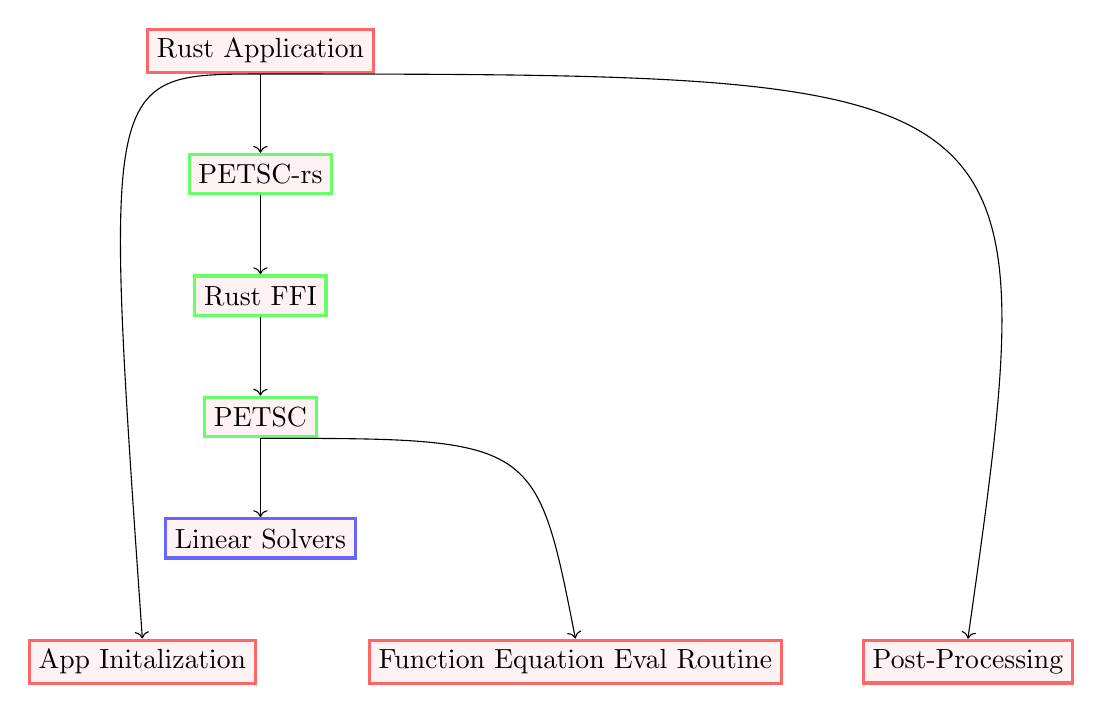
\begin{tikzpicture}[
	main/.style = {draw,circle},
	usercode/.style={rectangle, draw=red!60, fill=red!5, very thick, minimum size=5mm},
	librarycode/.style={rectangle, draw=green!60, fill=red!5, very thick, minimum size=5mm},
	linalgcode/.style={rectangle, draw=blue!60, fill=red!5, very thick, minimum size=5mm},
]
\node[usercode, align=center] (rust) {Rust Application};
\node[librarycode] (petsc-rs) [below=of rust]{PETSC-rs};
\node[librarycode] (rust-ffi) [below=of petsc-rs]{Rust FFI};
\node[librarycode] (petsc) [below=of rust-ffi]{PETSC};
\node[linalgcode] (solvers) [below=of petsc]{Linear Solvers};
\node[usercode] (callback) [below=of solvers, xshift=40mm]{Function Equation Eval Routine};
\node[usercode, align=center] (inital) [below=of solvers, xshift=-15mm]{App Initalization};
\node[usercode, align=center] (post) [right=of callback]{Post-Processing};

\draw[->](rust.south)--(petsc-rs.north);
\draw[->](petsc-rs.south)--(rust-ffi.north);
\draw[->](rust-ffi.south)--(petsc.north);
\draw[->](petsc.south) .. controls +(right:35mm) .. (callback.north);
\draw[->](rust.south) .. controls +(left:20mm) .. (inital.north);
\draw[->](rust.south) .. controls +(right:100mm) .. (post.north);
\draw[->](petsc.south)--(solvers);
\end{tikzpicture}\hspace{8mm}
\end{document}
